\Chapter{Tesztelés}

\Section{Natív és jQuery-vel történő kirajzolás}

A program megvalósításához szóba jött a Jquery használata is, és ezáltal az is, hogy vajon a Jquery-s vagy a sima context-re rajzolás lehet-e a gyorsabb.


Ehhez a vizsgálathoz két példa program is készült, az egyik azt vizsgálta, hogy melyik megoldás milyen gyorsasággal rajzol ki.

Nézzük a két kirajzolást. Amik a draw és a draw2 programban is megtalálhatóak.

\bigskip

\noindent jQuery:
\begin{java}
$('canvas').drawArc({
  strokeStyle: 'black',
  fillStyle: 'blue',
  strokeWidth: 2,
  x: 100, y: 200,
  radius: 50
});
\end{java}

\bigskip

\noindent Context:
\begin{java}
context.fillStyle = 'blue';
context.strokeStyle = 'black';
context.lineWidth = 2;
context.beginPath();
context.arc(200, 100, 50, 0, 2 * Math.PI);
context.fill();
context.stroke();
\end{java}

\medskip

1000-től 29000-ig vizsgáltuk a kirajzolást ezresével növelve a méretet, ugyanazzal a kitöltéssel, mérettel, és már itt láttuk, hogy a Jquery sokkal lassabb. Az itt kapott futási időket \aref{fig:pieces}. ábra tartalmazza.

\begin{figure}[h]
	\centering
	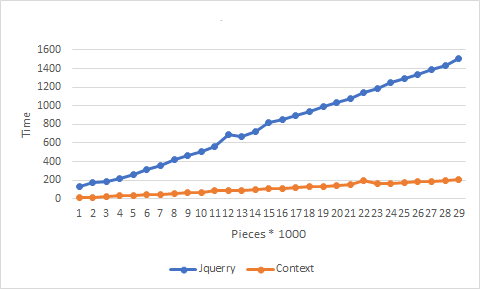
\includegraphics[width=\textwidth]{images/pieces.png}
	\caption{jQuery vs Context kirajzolás daraszám alapján.}
	\label{fig:pieces}
\end{figure}

\medskip

De vizsgáltunk egy másik szempontot is, még pedig, hogy ha a körök méretét növeljük, akkor melyik a gyorsabb. A fent említett kirajzolásokban, ez úgy jelent meg, hogy ahová a kör sugarát írtuk (ami ott 50 volt) oda egy betű változót írtunk, aminek utána az értékét változtattuk.

10-től 290-es méretig rajzoltattunk ki köröket tizesével növelve a méretet, és itt is láthattuk, hogy a Jquery lassabb, így a programban azt a megoldást nem használtuk. Az itt kapott futási időket pedig \aref{fig:radius}. ábra tartalmazza


\begin{figure}[h]
	\centering
	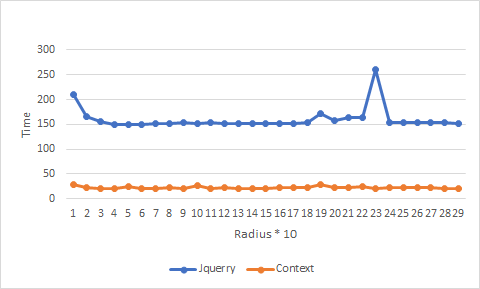
\includegraphics[width=\textwidth]{images/radius.png}
	\caption{jQuery vs Context kirajzolás méret alapján.}
	\label{fig:radius}
\end{figure}



\Section{Program használata}

A programok használata nagyon egyszerű, ha betöltött az oldal megjelennek a kis részecskék. Azokon kívül alul az előző fejezetben már bemutatott dolgokat látjuk (\ref{fig:html}. ábra). 

\textbf{Csúszkák}

A csúszkák segítségével a részecskékre ható erőket lehet módosítani. Ha jobbra húzzuk őket vagyis egyre több kék színt látunk, akkor azzal növeljük az értékeket. Ha balra vagyis egyre kevesebb kék színt látunk, azzal csökkentjük az értékeket. Az itt beállított értékeket, már az előbb is bemutatott módon folyamatosan nyomon követhetjük a képernyő bal felső sarkában (\ref{fig:ertekek} ábra). 


\textbf{Gombok}

A programban 2 gomb van ezek a pohár hozzáadás, illetve eltávolítás. A pohár hozzáadása gombbal egy poharat lehet a programhoz hozzáadni, az eltávolítóval meg nyilván eltávolítani. 

\textbf{Koordináták}

Az előzőleg említett gombokkal hozzáadott pohár koordinátáit lehet még módosítani a programban. Amik már szintén az előző fejezetben bemutatott módon hatnak a pohárra (\ref{fig:pohar} ábra). Itt be is írhatunk számokat, de ha az egérrel a számok fölé megyünk megjelenik egy felfelé és egy lefelé mutató nyíl, amikkel növelhetjük illetve csökkenthetjük az értékeket. 

\textbf{Követelmények}

A programnak nincs szüksége semmi másra csak egy webböngészőre. Ami a mai világban már szinte mindenre elérhető. 

\Section{Összehasonlítás}

Összehasonlítva a két programot láthatjuk, hogy melyik megoldás a jobb megoldás a részecske alapú víz ábrázolására. Ez pedig a kör alapú program, ugyanis hiába ugyanazon dolgok alapján mozognak a részecskék a körök máshogyan mozognak, egy idő után nincsenek állandó mozgásban, hanem szépen lassan lenyugszanak, ami a négyzet alapú programra nem igaz. Ott a négyzetek folyamatosan mozognak.
